% !TEX encoding = UTF-8 Unicode 
% !TEX root = praca.tex

\chapter{Projekt oraz implementacja rozwiązania}

\section{Wstęp}
W ramach pracy inżynierskiej opracowano kompleksowe narzędzie `gptester`, które wykorzystuje zaawansowane modele językowe do analizy statycznej kodu.
Narzędzie to wykorzystuje przede wszystkim model GPT-4 do generowania raportów na temat jakości kodu oraz proponowania poprawek, ze szczególnym uwzględnieniem bezpieczeństwa kodu.

\section{Architektura systemu}
\subsection{Ogólny opis}
`gptester` jest programem napisanym w języku Python, wykorzystującym model GPT-4 (lub GPT-3.5-turbo) dostarczony przez OpenAI. 
Jest zaprojektowany do uruchamiania z linii poleceń, a wyniki jego pracy są zapisywane w pliku formatu markdown oraz do osobnego katalogu z plikami wynikowymi - poprawionymi. 
W przyszłości planowane jest wprowadzanie poprawek do bazy kodu za pomocą git patch.

\subsection{Schemat blokowy}
\label{subsec:schemat_blokowy}

\begin{landscape}
\begin{figure}[p]
    \centering
    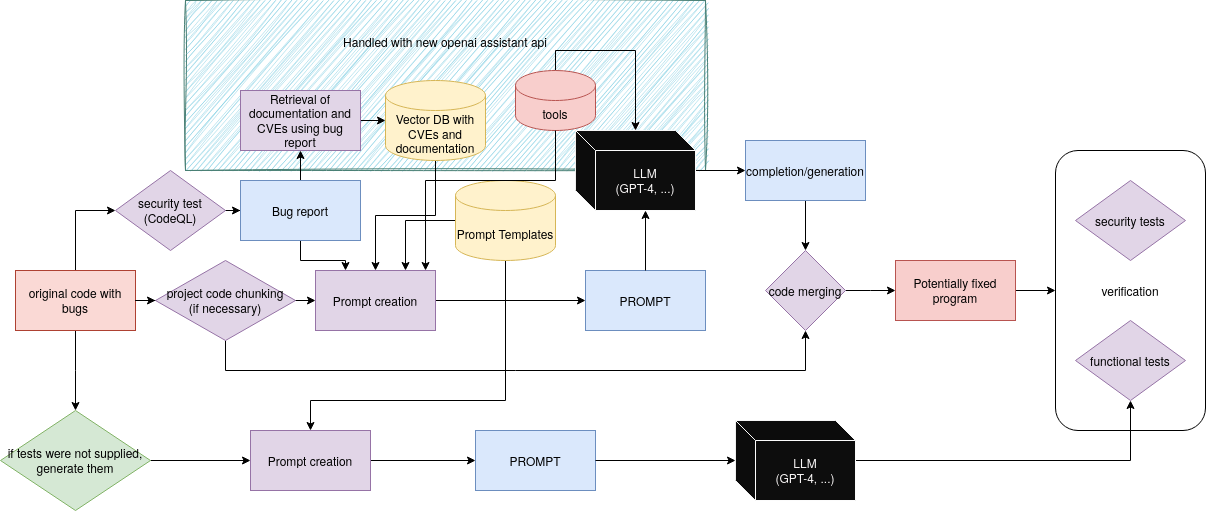
\includegraphics[width=\linewidth]{img/gptester.drawio.png}
    \caption{Schemat blokowy działania aplikacji `gptester`}
    \label{fig:schemat_blokowy}
\end{figure}
\end{landscape}

\section{Proces implementacji}
\subsection{Środowisko programistyczne i wymagania}
\label{sec:srodowisko_i_wymagania}

Projekt `gptester` został opracowany w środowisku programistycznym Python, z wykorzystaniem modelu GPT-4 dostarczonego przez OpenAI. Proces konfiguracji środowiska rozpoczyna się od przygotowania odpowiedniego środowiska Pythona i zainstalowania niezbędnych zależności.

Wymagania wstępne:
\begin{itemize}
    \item Python w wersji 3.x – Język programowania wykorzystany do napisania `gptester`.
    \item Dostęp do internetu – Niezbędny do pobrania zależności i interakcji z modelem GPT-4 przez API OpenAI.
\end{itemize}

Instalacja zależności:
\begin{listing}
    \begin{minted}{bash}
pip install -r requirements.txt
\end{minted}
\end{listing}

Plik `requirements.txt` zawiera wszystkie niezbędne biblioteki Pythona wymagane do działania `gptester`. Instalacja zależności jest prosta i może być wykonana w terminalu lub wirtualnym środowisku Pythona, co jest zalecane w celu uniknięcia konfliktów z istniejącymi pakietami.



\subsection{Funkcje programu}
\label{sec:funkcje_programu}

Program `gptester` został zaprojektowany jako wszechstronny narzędzie do analizy statycznej kodu, wykorzystując zaawansowane modele językowe do wykrywania i naprawiania błędów bezpieczeństwa w kodzie. Kluczowe funkcje programu są dostępne za pomocą różnorodnych argumentów linii poleceń, umożliwiając szeroką konfigurację i dostosowanie do specyicznych potrzeb analizy.

\begin{itemize}
    \item \textbf{-h, --help}: Wyświetla pomoc programu, zawierającą informacje o dostępnych opcjach i ich krótki opis. Jest to przydatne dla użytkowników, którzy chcą szybko zrozumieć, jak korzystać z programu.
    
    \item \textbf{-v, --verbose}: Aktywuje tryb szczegółowych informacji. W tym trybie, `gptester` wyświetla dodatkowe informacje na temat każdego etapu przetwarzania, co jest przydatne do debugowania i analizy szczegółów wykonania.
    
    \item \textbf{-m MODEL, --model MODEL}: Umożliwia wybór modelu językowego używanego do analizy kodu. Domyślnie ustawiony na "gpt-4-1106-preview", ale użytkownik może wybrać inny model, jeśli jest dostępny i lepiej odpowiada wymaganiom projektu.
    
    \item \textbf{-o OUTPUT, --output OUTPUT}: Określa ścieżkę i nazwę pliku, do którego będą zapisane wyniki analizy. Domyślnie, raport jest zapisywany w pliku markdown w folderze "raports" z nazwą opartą na nazwie analizowanego folderu i znaczniku czasowym. Użytkownik może dostosować tę lokalizację według własnych preferencji.

    \item \textbf{-t TESTS, --tests TESTS}: Pozwala na podanie ścieżki do testów funkcjonalnych, które mają zostać wykonane na analizowanym projekcie. Ta funkcja jest szczególnie przydatna w środowiskach, gdzie istnieje potrzeba zintegrowanego podejścia do testowania i analizy kodu.

    \item \textbf{-c, --codeql}: Włącza integrację z CodeQL, zaawansowanym narzędziem do analizy kodu. Użytkownik musi mieć zainstalowane CodeQL-CLI, aby skorzystać z tej funkcji. Jest to szczególnie przydatne w wykrywaniu bardziej złożonych problemów w kodzie, które mogą umknąć prostym analizom.

    \item \textbf{--command COMMAND}: Umożliwia określenie polecenia budującego projekt, co jest niezbędne dla prawidłowej integracji z CodeQL w przypadku, gdy projekt nie zawiera pliku cmake lub podobnego w katalogu głównym. Domyślnie ustawione na "make".

    \item \textbf{--language LANGUAGE}: Pozwala na określenie języka programowania projektu do analizy w CodeQL. Domyślnie ustawione na "cpp", ale można dostosować do innych języków wspieranych przez CodeQL, co rozszerza możliwości analizy na różnorodne środowiska programistyczne.

\end{itemize}

Przykład użycia z pełną konfiguracją:

\begin{listing}
    \begin{minted}{bash}
./main.py /ścieżka/do/projektu --verbose --model "gpt-4-1106-preview" --output "moj_raport.md" --tests "/ścieżka/do/testów" --codeql --command "cmake" --language "java"
\end{minted}
\end{listing}

W powyższym przykładzie, gptester analizuje kod znajdujący się w podanej ścieżce, z włączonym trybem szczegółowych informacji, korzystając z modelu GPT-4, zapisując wyniki do określonego pliku raportu, wykonując testy funkcjonalne, integrując z CodeQL, używając polecenia cmake do budowy projektu w języku Java.

\section{Integracja z CodeQL}
\label{sec:integracja_codeql}

Integracja `gptester` z CodeQL znacznie rozszerza jego funkcjonalność analizy statycznej kodu. CodeQL, opracowany przez GitHub, to zaawansowane narzędzie do semantycznej analizy kodu, które umożliwia wykrywanie złożonych podatności i błędów bezpieczeństwa.

\textbf{Główne cechy integracji z CodeQL:}
\begin{itemize}
    \item \textbf{Zaawansowana Analiza Bezpieczeństwa}: CodeQL przekształca kod źródłowy w zapytywalną formę, co pozwala na przeprowadzenie głębokich analiz w poszukiwaniu subtelnych luk bezpieczeństwa.
    \item \textbf{Wsparcie Dla Wielu Języków}: Obsługa różnych języków programowania przez CodeQL, takich jak C++, Java, Python, co jest wykorzystywane przez `gptester` do analizy różnorodnych projektów.
    \item \textbf{Konfiguracja Procesu Budowania}: Możliwość dostosowania polecenia budowania projektu za pomocą opcji \texttt{--command}, niezbędna w przypadku braku pliku konfiguracyjnego jak cmake w katalogu głównym.
    \item \textbf{Elastyczność Analizy}: Użytkownik może wybrać między szybkimi analizami a bardziej dogłębnymi badaniami, co umożliwia dostosowanie procesu do konkretnych wymagań projektu.
    \item \textbf{Automatyzacja Wykrywania Podatności}: CodeQL automatyzuje proces wykrywania podatności, zwiększając skuteczność i efektywność analizy bezpieczeństwa kodu.
\end{itemize}

Integracja z CodeQL czyni `gptester` narzędziem nie tylko do wykrywania błędów syntaktycznych i strukturalnych, ale także do efektywnego identyfikowania subtelniejszych problemów bezpieczeństwa, które mogą umknąć podczas standardowych analiz.

\section{Przypadki użycia}
\label{sec:przypadki_uzycia}

Przypadki użycia programu `gptester` demonstrują jego wszechstronność i elastyczność w różnych scenariuszach analizy kodu. Poniżej przedstawiono kilka przykładowych scenariuszy, które ilustrują, jak `gptester` może być wykorzystywany do osiągnięcia różnych celów w procesie analizy statycznej kodu.

\subsubsection{Podstawowa Analiza Kodu}
W najprostszym przypadku, `gptester` może być używany do przeprowadzenia podstawowej analizy kodu w określonym katalogu. Przykład użycia:

\begin{verbatim}
./main.py /ścieżka/do/projektu
\end{verbatim}

W tym scenariuszu, `gptester` przeanalizuje kod w podanym katalogu, używając domyślnych ustawień dla modelu językowego i zapisze raport w standardowej lokalizacji.

\subsubsection{Analiza z Wysokim Poziomem Detali}
Dla bardziej szczegółowych informacji, użytkownik może włączyć tryb verbose, co pozwoli na śledzenie szczegółowych informacji o każdym etapie analizy. Przykład użycia:

\begin{verbatim}
./main.py --verbose /ścieżka/do/projektu
\end{verbatim}

W tym przypadku, `gptester` dostarczy rozszerzone informacje o przeprowadzanej analizie, co jest szczególnie przydatne do debugowania i zrozumienia procesu analizy.

\subsubsection{Analiza z Integracją CodeQL}
Dla zaawansowanej analizy bezpieczeństwa, `gptester` może być używany w połączeniu z CodeQL. Przykład użycia:

\begin{verbatim}
./main.py --codeql --language java /ścieżka/do/projektu
\end{verbatim}

W tym scenariuszu, `gptester` wykorzystuje CodeQL do przeprowadzenia głębokiej analizy kodu w języku Java, co pozwala na wykrycie bardziej subtelnych i złożonych problemów bezpieczeństwa.

\subsubsection{Analiza Projektu z Konkretnym Modelem Językowym}
Użytkownik może również wybrać specyficzny model językowy dla analizy. Przykład użycia:

\begin{verbatim}
./main.py --model "gpt-4-1106-preview" /ścieżka/do/projektu
\end{verbatim}

Taki wybór modelu może być użyteczny, gdy użytkownik chce skorzystać z określonych cech lub możliwości danego modelu, które mogą być lepiej dostosowane do charakterystyki analizowanego kodu. 
W przyszłości wybór zostanie poszerzony o modele otwartoźródłowe nieograniczone narzuconymi limitami OpenAI.

\subsubsection{Kompleksowa Analiza z Wykorzystaniem Testów Funkcjonalnych}
gptester pozwala na integrację testów funkcjonalnych, co może być użyteczne do bardziej kompleksowej analizy projektu. Przykład użycia:

\begin{verbatim}
./main.py --tests "/ścieżka/do/testów" /ścieżka/do/projektu
\end{verbatim}

W tym przypadku, oprócz standardowej analizy kodu, gptester wykonuje również testy funkcjonalne, co pozwala na lepsze zrozumienie, jak zmiany w kodzie wpływają na działanie aplikacji.

\subsubsection{Zaawansowana Konfiguracja dla Specyficznych Wymagań}
Dla projektów o specyficznych wymaganiach, gptester oferuje szeroki zakres opcji konfiguracyjnych, pozwalając na dostosowanie analizy do indywidualnych potrzeb. Przykład użycia:

\begin{verbatim}
./main.py --verbose --model "gpt-4-1106-preview" --output "moj_raport.md" --tests "/ścieżka/do/testów" --codeql --command "cmake" --language "java" /ścieżka/do/projektu
\end{verbatim}

Tutaj, gptester jest konfigurowany do pracy z konkretnym modelem językowym, zapisuje raport w określonym pliku, wykonuje testy funkcjonalne, integruje z CodeQL, korzysta z określonego polecenia budowania projektu i jest dostosowany do analizy kodu w języku Java.
\begin{listing}
    \begin{minted}{c}  
Przykład użycia podstawowego

cd gptester
python main.py -h
Przykład użycia z opcją verbose

./main.py --verbose
Przykład użycia z integracją CodeQL

./main.py --codeql --command "make" --language "cpp"
    \end{minted}
    \caption{Przykłady użycia programu gptester}
    \label{lst:przyklady_uzycia}
\end{listing}

\section{Rozwój i plany na przyszłość}
\label{sec:rozwoj_i_plany_na_przyszlosc}

Sekcja ta skupia się na omówieniu obecnego stanu projektu `gptester` oraz planowanych rozszerzeń i ulepszeń, które mają zostać wprowadzone w przyszłości. Planowane działania są zgodne z informacjami zawartymi w sekcji "In development" w README.md.

\subsection{Obecne osiągnięcia}
\label{subsec:obecne_osiagniecia}

Projekt `gptester` osiągnął już kilka kluczowych kamieni milowych w swoim rozwoju:

\begin{itemize}
    \item \textbf{Podstawowa funkcjonalność}: Program już teraz oferuje podstawowe funkcje analizy statycznej kodu, umożliwiając identyfikację typowych błędów i podatności.
    \item \textbf{Wykorzystanie technik RAG oraz in-context learning}: `gptester` wykorzystuje zaawansowane techniki generacji wspomaganej odzyskiwaniem danych oraz uczenia się w kontekście, co pozwala na lepsze dostosowanie modeli językowych do specyficznych zadań.
    \item \textbf{Integracja z CodeQL}: Znaczącym osiągnięciem jest wdrożenie integracji z CodeQL, co znacznie rozszerza możliwości analizy kodu, szczególnie w zakresie wykrywania złożonych błędów bezpieczeństwa.
\end{itemize}

Te osiągnięcia stanowią solidną podstawę dla dalszego rozwoju i rozbudowy `gptester`, kładąc nacisk na wydajność, dokładność i wszechstronność narzędzia.

\subsection{Planowane rozszerzenia}
\label{subsec:planowane_rozszerzenia}

W ramach dalszego rozwoju, projekt `gptester` ma w planach kilka istotnych rozszerzeń i ulepszeń:

\begin{itemize}
    \item \textbf{Aktualizacja kodu za pomocą funkcji git i plików patch}: Rozwój funkcjonalności, która pozwoli na automatyczne wprowadzanie poprawek do kodu źródłowego na podstawie wygenerowanych plików git i patch. To ulepszenie ułatwi proces naprawy kodu, umożliwiając automatyczne aplikowanie poprawek oraz interaktywne wybieranie elementów z obu wersji.
    \item \textbf{Dodanie więcej testów oraz automatyzacja testów bezpieczeństwa}: Rozbudowa zestawu testów funkcjonalnych, jednostkowych i bezpieczeństwa, co pozwoli na lepsze sprawdzanie niezawodności i efektywności `gptester`. Automatyzacja testów pozwoli na skuteczniejsze wykrywanie błędów oraz ułatwi badania.
    \item \textbf{Obsługa więcej języków programowania dla CodeQL}: Rozszerzenie integracji z CodeQL o więcej języków programowania, co zwiększy użyteczność `gptester` w różnorodnych projektach programistycznych. Planowane jest dodanie wsparcia dla popularnych języków takich jak JavaScript, Python czy Ruby.
\end{itemize}

Te planowane rozszerzenia mają na celu nie tylko ulepszenie obecnych funkcjonalności gptester, ale również wprowadzenie nowych możliwości, które uczynią narzędzie jeszcze bardziej wszechstronnym i przydatnym w różnych kontekstach analizy kodu.
\section{Podsumowanie}
\label{sec:podsumowanie}

W niniejszym rozdziale przedstawiono szczegółowy opis projektu `gptester`, jego obecne możliwości oraz plany rozwojowe. `gptester`, jako zaawansowane narzędzie do analizy statycznej kodu, wykorzystujące model GPT-4 od OpenAI, stanowi znaczący krok naprzód w dziedzinie automatyzacji i poprawy jakości kodu źródłowego.

\textbf{Podstawowe osiągnięcia:}
\begin{itemize}
    \item Rozwój podstawowych funkcjonalności analizy statycznej, umożliwiających efektywne wykrywanie i naprawianie błędów w kodzie.
    \item Integracja z CodeQL, dzięki której `gptester` zyskuje zdolność do przeprowadzania bardziej zaawansowanych analiz bezpieczeństwa.
    \item Elastyczność w obsłudze różnorodnych scenariuszy użytkowania poprzez konfigurowalne argumenty linii poleceń.
\end{itemize}

\textbf{Plany rozwojowe:}
\begin{itemize}
    \item Rozbudowa funkcjonalności aktualizacji kodu źródłowego za pomocą plików git i patch, co uprości proces wprowadzania poprawek.
    \item Dodanie wsparcia dla dodatkowych języków programowania w integracji z CodeQL, co rozszerzy zakres zastosowania `gptester`.
    \item Automatyzacja testów.
\end{itemize}

Podsumowując, `gptester` już teraz stanowi potężne narzędzie do analizy i poprawy kodu źródłowego, a planowane rozbudowy i ulepszenia sprawią, że będzie ono jeszcze bardziej wszechstronne i skuteczne. Projekt ten pokazuje, jak technologie AI i narzędzia do automatycznej analizy kodu mogą przyczynić się do poprawy jakości oprogramowania oraz efektywności procesów programistycznych.
